\documentclass{article}
% generated by Madoko, version 1.1.3
%mdk-data-line={1}


\usepackage[heading-base={2},section-num={False},bib-label={hide},fontspec={True}]{madoko2}
\usepackage[UTF8]{ctex}
\usepackage{parskip}
\usepackage[left=2.5cm,right=2.5cm,top=3cm,bottom=3cm]{geometry}
%mdk-data-line={5}
\setlength{\parindent}{0cm}

\begin{document}



%mdk-data-line={11}
\mdxtitleblockstart{}
%mdk-data-line={11}
\mdxtitle{\mdline{11}软工课设题目}%mdk
\mdxauthorstart{}
%mdk-data-line={16}
\mdxauthorname{\mdline{16}张盛强}%mdk

%mdk-data-line={19}
\mdxauthoremail{\mdline{19}zhangsq5829@gmail.com}%mdk
\mdxauthorend
%mdk-data-line={28}
\mdxtitlefooter{\mdline{28}2017-05-26}%mdk
\mdtitleauthorrunning{}{}\mdxtitleblockend%mdk

%mdk-data-line={13}
\section{\mdline{13}1.\hspace*{0.5em}\mdline{13}Problem Statement问题描述}\label{sec-problem-statement}%mdk%mdk

%mdk-data-line={15}
\noindent\mdline{15}作为Acme公司的领导,你接到一项任务:建立一个新的工资单系统去取代原有的系统,原有的系统已经非常过时了。Acme现在需要一个新的系统来允许员工记录考勤信息(\mdline{15}\mdcode{timecard~information}\mdline{15}),并且能根据工作时长和销售业绩来自动产生薪水(\mdline{15}\mdcode{paychecks}\mdline{15})(for commissioned employees)。%mdk

%mdk-data-line={18}
\mdline{18}新的系统必须是最新技术的,并且有一个基于Windows的桌面接口,来允许员工进入员工考勤信息界面,进入购买订单界面,改变员工喜好(例如支付方式),并且创建不同的报告。这个系统贯穿整个公司,运行在员工个人的桌面上。出于安全和查账的原因,雇员们只能访问并编辑属于他们自己的考勤信息和购买订单。%mdk

%mdk-data-line={20}
\mdline{20}系统会保留公司所有员工的信息(Acme现在全球范围内拥有5000名员工)。系统必须能够按时支付每位员工正确的数目金钱(用他们个人喜欢的领工资方法)。Acme出于价格的考虑,不想替换他们遗留的一个数据库,工程管理数据库(the Project Management Database),它包含关于工程(Projects)和费用(charge numbers)的所有信息。新的系统必须和已有的Project Management Database协同工作,这是一个工作在IBM主机上的DB2数据库。工资单系统可以访问,但是不能更新存储在Project Management Database中的数据。%mdk

%mdk-data-line={22}
\mdline{22}一些员工按小时工作,所以他们就按照小时来计算工资。他们提交记录着日期(date)和为某特定\mdline{22}\mdcode{charge~number}\mdline{22}工作小时数的考勤卡(timecards)。如果有人工作超过8小时,那么Acme会为他们超过8小时的工作时间部分支付他们一般每小时工钱的1.5倍工资。按小时支付的员工每周五发工资。%mdk

%mdk-data-line={24}
\mdline{24}一些员工以固定薪水支付工资。即使是按固定工资支付的,他们也需要提交记录着日期和工作小时的考勤卡。这样系统可以追踪他们为特定\mdline{24}\mdcode{charge~~number}\mdline{24}工作的小时数。这些人在每个月的最后一个工作日领工资。%mdk

%mdk-data-line={26}
\mdline{26}一些有薪水的员工也接受基于他们销售量的佣金(commission)。他们提交反映了日期和销售额的购买订单(purchase orders),\mdline{26}\mdcode{commission~rate}\mdline{26} 根据每个员工的情况而定,\mdline{26}\mdcode{Commission~rate}\mdline{26}是 10\%,15\%,25\%,35\%的其中之一。%mdk

%mdk-data-line={28}
\mdline{28}新系统最迫切需要的一个特色是能生成员工报告(Employee reporting),员工能在系统上查询工作时长,为某个项目(即charge number)付出的总时长,年初至今收到的总工资,剩余的假期时间,等等。%mdk

%mdk-data-line={30}
\mdline{30}员工可以选择他们的支付方式。他们可以选择将他们的薪水支票邮寄到他们提交的地址,他们也可以要求直接存款并且将存款存进他们选择的银行账户。员工也可以选择在办公室直接拿走薪水支票。%mdk

%mdk-data-line={32}
\mdline{32}工资单管理员维护着员工信息。工资单管理者对以下事务负有职责:添加新员工,删除员工,更改员工信息例如姓名,地址,雇佣方式(小时制,薪水制,委任制),也包括运行管理报告(running administrative reports)。%mdk

%mdk-data-line={34}
\mdline{34}工资单应用程序会自动在每周五和当月的最后一个工作日工作。它会在这些日子里支付工资给适当的员工。这个系统会被告诉在哪天要付给员工工资,因此它会生成支付记录,该记录涵盖从最近一次支付的日期到特定的日期。新的系统这样设计是为了工资单总是可以自动生成,而不用任何人工干预。%mdk

%mdk-data-line={36}
\section{\mdline{36}2.\hspace*{0.5em}\mdline{36}Glossary术语表}\label{sec-glossary}%mdk%mdk

%mdk-data-line={37}
\subsection{\mdline{37}2.1.\hspace*{0.5em}\mdline{37}Introduction}\label{sec-introduction}%mdk%mdk

%mdk-data-line={38}
\noindent\mdline{38}这篇文档是为特定问题领域,解释项定义的术语,这些术语可能对用例描述和其他项目文档的阅读者来说不熟悉。这篇文档常常被当做非正式的数据字典来使用,抓住数据定义使得用例描述和其他项目文档可以更加集中于系统必须做什么。%mdk

%mdk-data-line={40}
\subsection{\mdline{40}2.2.\hspace*{0.5em}\mdline{40}Definitions}\label{sec-definitions}%mdk%mdk

%mdk-data-line={41}
\noindent\mdline{41}这篇术语表包含工资单系统中关键概念的\mdline{41}\mdcode{working~~definitions}\mdline{41}。%mdk

%mdk-data-line={43}
\subsection{\mdline{43}2.3.\hspace*{0.5em}\mdline{43}Bank System}\label{sec-bank-system}%mdk%mdk

%mdk-data-line={44}
\noindent\mdline{44}直接存款交易所涉及的一切银行%mdk

%mdk-data-line={46}
\subsection{\mdline{46}2.4.\hspace*{0.5em}\mdline{46}Employee}\label{sec-employee}%mdk%mdk

%mdk-data-line={47}
\noindent\mdline{47}为公司工作的人,他们拥有并操作工资单系统%mdk

%mdk-data-line={49}
\subsection{\mdline{49}2.5.\hspace*{0.5em}\mdline{49}Payroll Administrator}\label{sec-payroll-administrator}%mdk%mdk

%mdk-data-line={50}
\noindent\mdline{50}负责维护员工和员工信息的人%mdk

%mdk-data-line={52}
\subsection{\mdline{52}2.6.\hspace*{0.5em}\mdline{52}Project Management Database}\label{sec-project-management-database}%mdk%mdk

%mdk-data-line={53}
\noindent\mdline{53}包含项目和charge numbers所有信息的遗留数据库%mdk

%mdk-data-line={55}
\subsection{\mdline{55}2.7.\hspace*{0.5em}\mdline{55}System Clock}\label{sec-system-clock}%mdk%mdk

%mdk-data-line={56}
\noindent\mdline{56}内部追踪时间的系统时钟,这个内部始终会在合适的时间自动地运行工资单系统%mdk

%mdk-data-line={58}
\subsection{\mdline{58}2.8.\hspace*{0.5em}\mdline{58}Pay Period}\label{sec-pay-period}%mdk%mdk

%mdk-data-line={59}
\noindent\mdline{59}一个员工已经被支付的总时间%mdk

%mdk-data-line={61}
\subsection{\mdline{61}2.9.\hspace*{0.5em}\mdline{61}Paycheck}\label{sec-paycheck}%mdk%mdk

%mdk-data-line={62}
\noindent\mdline{62}在一个特定的Pay Period内一个员工被支付的工资数目的记录%mdk

%mdk-data-line={64}
\subsection{\mdline{64}2.10.\hspace*{0.5em}\mdline{64}Payment Method}\label{sec-payment-method}%mdk%mdk

%mdk-data-line={65}
\noindent\mdline{65}员工被支付的方式,有现取,邮寄,直接存储。%mdk

%mdk-data-line={67}
\subsection{\mdline{67}2.11.\hspace*{0.5em}\mdline{67}Timecard}\label{sec-timecard}%mdk%mdk

%mdk-data-line={68}
\noindent\mdline{68}在一个特定的Pay Period期间员工工作时长的记录%mdk

%mdk-data-line={70}
\subsection{\mdline{70}2.12.\hspace*{0.5em}\mdline{70}Purchase Order}\label{sec-purchase-order}%mdk%mdk

%mdk-data-line={71}
\noindent\mdline{71}一个员工的销售记录%mdk

%mdk-data-line={73}
\subsection{\mdline{73}2.13.\hspace*{0.5em}\mdline{73}Salaried Employee}\label{sec-salaried-employee}%mdk%mdk

%mdk-data-line={74}
\noindent\mdline{74}接受薪水的员工%mdk

%mdk-data-line={76}
\subsection{\mdline{76}2.14.\hspace*{0.5em}\mdline{76}Commissionded Employee}\label{sec-commissionded-employee}%mdk%mdk

%mdk-data-line={77}
\noindent\mdline{77}接受薪水+提成的员工%mdk

%mdk-data-line={79}
\subsection{\mdline{79}2.15.\hspace*{0.5em}\mdline{79}Hourly Employee}\label{sec-hourly-employee}%mdk%mdk

%mdk-data-line={80}
\noindent\mdline{80}按小时支付的员工%mdk

%mdk-data-line={82}
\section{\mdline{82}3.\hspace*{0.5em}\mdline{82}Supplementary Specification补充说明}\label{sec-supplementary-specification}%mdk%mdk

%mdk-data-line={83}
\subsection{\mdline{83}3.1.\hspace*{0.5em}\mdline{83}Objectives目的}\label{sec-objectives}%mdk%mdk

%mdk-data-line={84}
\noindent\mdline{84}这篇文档的目的是定义工资单系统的需求。补充说明列出了没有在用例模型的用例中列出的要求。这篇补充说明和用例模型一起组成这个系统需求的完备集。%mdk

%mdk-data-line={86}
\subsection{\mdline{86}3.2.\hspace*{0.5em}\mdline{86}Scope范围}\label{sec-scope}%mdk%mdk

%mdk-data-line={87}
\noindent\mdline{87}这份补充说明适用于OOAD学生开发的工资单系统。%mdk

%mdk-data-line={89}
\mdline{89}这份说明定义了系统的非功能性需求,比如可靠性,实用性,性能,可支持性,也包括一些在用例间通用的功能性需求。(功能性需求在用例说明中)%mdk

%mdk-data-line={91}
\subsection{\mdline{91}3.3.\hspace*{0.5em}\mdline{91}References}\label{sec-references}%mdk%mdk

%mdk-data-line={92}
\noindent\mdline{92}None%mdk

%mdk-data-line={94}
\subsection{\mdline{94}3.4.\hspace*{0.5em}\mdline{94}Functionality}\label{sec-functionality}%mdk%mdk

%mdk-data-line={95}
\noindent\mdline{95}None%mdk

%mdk-data-line={97}
\subsection{\mdline{97}3.5.\hspace*{0.5em}\mdline{97}Usability}\label{sec-usability}%mdk%mdk

%mdk-data-line={98}
\noindent\mdline{98}None%mdk

%mdk-data-line={100}
\subsection{\mdline{100}3.6.\hspace*{0.5em}\mdline{100}Reliability}\label{sec-reliability}%mdk%mdk

%mdk-data-line={101}
\noindent\mdline{101}主要的系统98\%的时间都在运行。工资单在运行时系统是开机的并且在运行,这是很必要的。(每个周五以及当月的最后一个工作日)%mdk

%mdk-data-line={103}
\subsection{\mdline{103}3.7.\hspace*{0.5em}\mdline{103}Performance}\label{sec-performance}%mdk%mdk

%mdk-data-line={104}
\noindent\mdline{104}这个系统必须能够允许同时有2000个用户在任何时间访问中央数据库,500个用户在任何一个时间访问本地数据库。%mdk

%mdk-data-line={106}
\subsection{\mdline{106}3.8.\hspace*{0.5em}\mdline{106}Supportability}\label{sec-supportability}%mdk%mdk

%mdk-data-line={107}
\noindent\mdline{107}None%mdk

%mdk-data-line={109}
\subsection{\mdline{109}3.9.\hspace*{0.5em}\mdline{109}Security}\label{sec-security}%mdk%mdk

%mdk-data-line={110}
\noindent\mdline{110}这个系统必须能防止员工更改除自己以外的其他任何人的考勤记录。另外,出于安全考虑,只有工资单管理员被允许更改任意员工的信息with the exception of the payment delivery method.%mdk

%mdk-data-line={112}
\subsection{\mdline{112}3.10.\hspace*{0.5em}\mdline{112}Design Constraints}\label{sec-design-constraints}%mdk%mdk

%mdk-data-line={113}
\noindent\mdline{113}这个系统应该和已经存在的遗留系统\mdline{113}\mdcode{the~Project~Management~Database}\mdline{113}融为一体。这个遗留系统是一个工作在IBM主机上的DB2数据库。%mdk

%mdk-data-line={115}
\mdline{115}这个系统应该通过一个电子交易接口和已有的银行系统产生联系,(NOTE:外部银行系统的一般接口需要在这个过程早期被定义并且在这里定义 或者 在一个分开的支持性文档中。比如说不在这门课范围内的一个定义)%mdk

%mdk-data-line={117}
\mdline{117}这个系统需要提供一个基于Windows的桌面接口。%mdk

%mdk-data-line={119}
\section{\mdline{119}4.\hspace*{0.5em}\mdline{119}Use-Case model}\label{sec-use-case-model}%mdk%mdk

%mdk-data-line={120}
\subsection{\mdline{120}4.1.\hspace*{0.5em}\mdline{120}Payroll System Use-Case Model Main Diagram}\label{sec-payroll-system-use-case-model-main-diagram}%mdk%mdk

%mdk-data-line={121}
\noindent\mdline{121}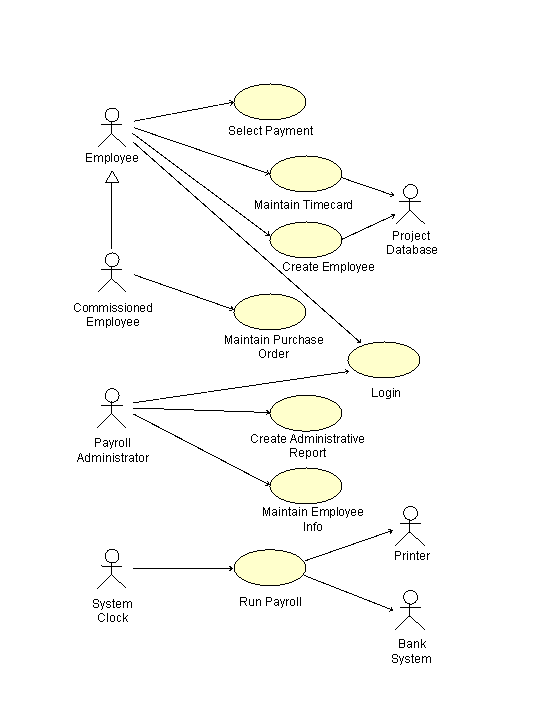
\includegraphics[keepaspectratio=true,width=\dimmin{}{\dimwidth{0.90}}]{images/-}{}\mdline{121}%mdk

%mdk-data-line={125}
\subsection{\mdline{125}4.2.\hspace*{0.5em}\mdline{125}Create Administrative Report}\label{sec-create-administrative-report}%mdk%mdk

%mdk-data-line={126}
\subsubsection{\mdline{126}4.2.1.\hspace*{0.5em}\mdline{126}Brief Description}\label{sec-brief-description}%mdk%mdk

%mdk-data-line={127}
\noindent\mdline{127}用例允许工资单管理员创建\mdline{127}\mdcode{Total~Hours~Worked}\mdline{127}或\mdline{127}\mdcode{Pay~Year-to-Date}\mdline{127}报告。%mdk

%mdk-data-line={129}
\subsubsection{\mdline{129}4.2.2.\hspace*{0.5em}\mdline{129}Flow of Events 事件流}\label{sec-flow-of-events-}%mdk%mdk

%mdk-data-line={130}
\paragraph{\mdline{130}4.2.2.1.\hspace*{0.5em}\mdline{130}\emph{Basic Flow}}\label{sec-_basic-flow_}%mdk%mdk

%mdk-data-line={132}
\noindent\mdline{132}\mdbr
\mdline{133}当工资单管理员请求系统生成管理报告时用例开始。%mdk

%mdk-data-line={134}
\begin{enumerate}%mdk

%mdk-data-line={134}
\item{}
%mdk-data-line={134}
\mdline{134}系统请求工资单管理员详细说明以下报告标准:%mdk

%mdk-data-line={135}
\begin{itemize}[noitemsep,topsep=\mdcompacttopsep]%mdk

%mdk-data-line={135}
\item\mdline{135}Report Type(total hours or pay Year-to-Date)%mdk

%mdk-data-line={136}
\item\mdline{136}Begin and end dates for the Report%mdk

%mdk-data-line={137}
\item\mdline{137}Employee name(s)%mdk
%mdk
\end{itemize}%mdk%mdk

%mdk-data-line={139}
\item{}
%mdk-data-line={139}
\mdline{139}一旦工资单管理员提供了要求的信息,系统就可以提供一份满足报告要求的报告。%mdk%mdk

%mdk-data-line={141}
\item{}
%mdk-data-line={141}
\mdline{141}工资单管理员可能在稍后会请求保存报告。与此同时,系统会要求工资单管理员提供保存报告所需的名字和存储位置。%mdk%mdk

%mdk-data-line={143}
\item{}
%mdk-data-line={143}
\mdline{143}一旦工资单管理员提供了要求的信息并且做出了保存报告的决定,系统就会以特定的名字在特定的存储位置保存报告。%mdk%mdk

%mdk-data-line={145}
\item{}
%mdk-data-line={145}
\mdline{145}如果工资单管理员没有选择保存报告,则该报告将会被丢弃。%mdk%mdk
%mdk
\end{enumerate}%mdk

%mdk-data-line={147}
\paragraph{\mdline{147}4.2.2.2.\hspace*{0.5em}\mdline{147}\emph{Alternative Flows}}\label{sec-_alternative-flows_}%mdk%mdk

%mdk-data-line={149}
\begin{itemize}%mdk

%mdk-data-line={149}
\item{}
%mdk-data-line={149}
\mdline{149}Requested Information Unavailable%mdk

%mdk-data-line={151}
\mdline{151}如果在\mdline{151}\mdcode{Basic~Flow}\mdline{151}中,请求的信息没有满足,系统将会给出错误信息。工资单管理员可以选择:%mdk

%mdk-data-line={152}
\begin{itemize}[noitemsep,topsep=\mdcompacttopsep]%mdk

%mdk-data-line={152}
\item\mdline{152}要么会退到\mdline{152}\mdcode{Basic~Flow}\mdline{152}的开始,%mdk

%mdk-data-line={153}
\item\mdline{153}要么在用例结束点取消操作%mdk
%mdk
\end{itemize}%mdk%mdk

%mdk-data-line={155}
\item{}
%mdk-data-line={155}
\mdline{155}Invalid Format or Insufficient Information%mdk

%mdk-data-line={157}
\mdline{157}如果在\mdline{157}\mdcode{Basic~Flow}\mdline{157}中,工资单管理员没有足够的特定信息去创建选择的报告,系统会提示缺失的信息。工资单管理员可以:%mdk

%mdk-data-line={158}
\begin{itemize}[noitemsep,topsep=\mdcompacttopsep]%mdk

%mdk-data-line={158}
\item\mdline{158}要么进入缺失信息%mdk

%mdk-data-line={159}
\item\mdline{159}要么选择在用例结束点取消操作%mdk
%mdk
\end{itemize}%mdk%mdk
%mdk
\end{itemize}%mdk

%mdk-data-line={161}
\subsubsection{\mdline{161}4.2.3.\hspace*{0.5em}\mdline{161}Special Requirements}\label{sec-special-requirements}%mdk%mdk

%mdk-data-line={162}
\noindent\mdline{162}None%mdk

%mdk-data-line={164}
\subsubsection{\mdline{164}4.2.4.\hspace*{0.5em}\mdline{164}Pre-Conditions}\label{sec-pre-conditions}%mdk%mdk

%mdk-data-line={165}
\noindent\mdline{165}工资单管理员必须得登录进系统,使得用例开始。%mdk

%mdk-data-line={167}
\subsubsection{\mdline{167}4.2.5.\hspace*{0.5em}\mdline{167}Post-Conditions}\label{sec-post-conditions}%mdk%mdk

%mdk-data-line={168}
\noindent\mdline{168}系统状态不会被用例改变%mdk

%mdk-data-line={170}
\subsubsection{\mdline{170}4.2.6.\hspace*{0.5em}\mdline{170}Extension Points}\label{sec-extension-points}%mdk%mdk

%mdk-data-line={171}
\noindent\mdline{171}None%mdk

%mdk-data-line={173}
\subsection{\mdline{173}4.3.\hspace*{0.5em}\mdline{173}Create Employee Report}\label{sec-create-employee-report}%mdk%mdk

%mdk-data-line={174}
\subsubsection{\mdline{174}4.3.1.\hspace*{0.5em}\mdline{174}Brief Description}\label{sec-brief-description}%mdk%mdk

%mdk-data-line={175}
\noindent\mdline{175}用例允许员工创建一个以下类型的报告:%mdk

%mdk-data-line={177}
\begin{itemize}[noitemsep,topsep=\mdcompacttopsep]%mdk

%mdk-data-line={177}
\item\mdline{177}\mdcode{Total~Hours~Worked}\mdline{177},%mdk

%mdk-data-line={178}
\item\mdline{178}\mdcode{Total~Hours~Worked~for~a~Project}\mdline{178},%mdk

%mdk-data-line={179}
\item\mdline{179}\mdcode{Vacation/Sick~Leave}\mdline{179},%mdk

%mdk-data-line={180}
\item\mdline{180}\mdcode{Total~Pay~Year-to-Date}\mdline{180}.%mdk
%mdk
\end{itemize}%mdk

%mdk-data-line={182}
\subsubsection{\mdline{182}4.3.2.\hspace*{0.5em}\mdline{182}Flow of Events}\label{sec-flow-of-events}%mdk%mdk

%mdk-data-line={183}
\paragraph{\mdline{183}4.3.2.1.\hspace*{0.5em}\mdline{183}\emph{Basic Flow}}\label{sec-_basic-flow_}%mdk%mdk

%mdk-data-line={185}
\noindent\mdline{185}\mdbr
\mdline{186}在员工希望创建以上4中类型报告之一时,用例开始。%mdk

%mdk-data-line={187}
\begin{enumerate}[noitemsep,topsep=\mdcompacttopsep]%mdk

%mdk-data-line={187}
\item\mdline{187}系统要求员工详细说明下列报告标准:

%mdk-data-line={188}
\begin{itemize}[noitemsep,topsep=\mdcompacttopsep]%mdk

%mdk-data-line={188}
\item\mdline{188}Report Type(以上4中类型之一)%mdk

%mdk-data-line={189}
\item\mdline{189}Begin and end dates for the report%mdk
%mdk
\end{itemize}%mdk%mdk

%mdk-data-line={190}
\item\mdline{190}若员工选择\mdline{190}\mdcode{Total~Hours~Worked~for~a~Project}\mdline{190}报告时,系统会从\mdline{190}\mdcode{Project~Management~Database}\mdline{190}中检索并展示一列可用的\mdline{190}\mdcode{charge~numbers}\mdline{190},然后系统会要求员工选择一个\mdline{190}\mdcode{charge~number}\mdline{190}%mdk

%mdk-data-line={191}
\item\mdline{191}一旦员工提供了必要的信息,系统就会生成满足报告标准的报告。%mdk

%mdk-data-line={192}
\item\mdline{192}员工稍后可能会请求系统保存报告。这时,系统会要求员工提供报告的名字和存储位置。%mdk

%mdk-data-line={193}
\item\mdline{193}一旦员工提供了要求的信息并且做出了保存报告的决定,系统就会以特定的名字在特定的存储位置保存报告。%mdk

%mdk-data-line={194}
\item\mdline{194}如果员工没有选择保存报告,则报告会被丢弃。%mdk
%mdk
\end{enumerate}%mdk

%mdk-data-line={196}
\paragraph{\mdline{196}4.3.2.2.\hspace*{0.5em}\mdline{196}\emph{Alternative Flows}}\label{sec-_alternative-flows_}%mdk%mdk

%mdk-data-line={197}
\begin{itemize}%mdk

%mdk-data-line={197}
\item{}
%mdk-data-line={197}
\mdline{197}Requested Information Unavailable%mdk

%mdk-data-line={199}
\mdline{199}如果在\mdline{199}\mdcode{Basic~Flow}\mdline{199}中,请求的信息没有满足,系统将会给出错误信息。员工可以选择:%mdk

%mdk-data-line={200}
\begin{itemize}[noitemsep,topsep=\mdcompacttopsep]%mdk

%mdk-data-line={200}
\item\mdline{200}要么会退到\mdline{200}\mdcode{Basic~Flow}\mdline{200}的开始,%mdk

%mdk-data-line={201}
\item\mdline{201}要么在用例结束点取消操作%mdk
%mdk
\end{itemize}%mdk%mdk
%mdk
\end{itemize}%mdk

%mdk-data-line={204}
\begin{itemize}%mdk

%mdk-data-line={204}
\item{}
%mdk-data-line={204}
\mdline{204}Invalid Format or Insufficient Information%mdk

%mdk-data-line={206}
\mdline{206}如果在\mdline{206}\mdcode{Basic~Flow}\mdline{206}中,员工没有足够的特定信息去创建选择的报告,系统会提示缺失的信息。员工可以:%mdk

%mdk-data-line={207}
\begin{itemize}[noitemsep,topsep=\mdcompacttopsep]%mdk

%mdk-data-line={207}
\item\mdline{207}要么进入缺失信息%mdk

%mdk-data-line={208}
\item\mdline{208}要么选择在用例结束点取消操作%mdk
%mdk
\end{itemize}%mdk%mdk
%mdk
\end{itemize}%mdk

%mdk-data-line={210}
\subsubsection{\mdline{210}4.3.3.\hspace*{0.5em}\mdline{210}Special Events}\label{sec-special-events}%mdk%mdk

%mdk-data-line={211}
\noindent\mdline{211}None%mdk

%mdk-data-line={213}
\subsubsection{\mdline{213}4.3.4.\hspace*{0.5em}\mdline{213}Pre-Conditions}\label{sec-pre-conditions}%mdk%mdk

%mdk-data-line={214}
\noindent\mdline{214}在用例开始前,员工必须登录进系统。%mdk

%mdk-data-line={216}
\subsubsection{\mdline{216}4.3.5.\hspace*{0.5em}\mdline{216}Post-Conditions}\label{sec-post-conditions}%mdk%mdk

%mdk-data-line={217}
\noindent\mdline{217}系统的状态不会被用例改变%mdk

%mdk-data-line={219}
\subsubsection{\mdline{219}4.3.6.\hspace*{0.5em}\mdline{219}Extension Points}\label{sec-extension-points}%mdk%mdk

%mdk-data-line={220}
\noindent\mdline{220}None%mdk

%mdk-data-line={222}
\subsection{\mdline{222}4.4.\hspace*{0.5em}\mdline{222}Login}\label{sec-login}%mdk%mdk

%mdk-data-line={223}
\subsubsection{\mdline{223}4.4.1.\hspace*{0.5em}\mdline{223}Brief Description}\label{sec-brief-description}%mdk%mdk

%mdk-data-line={224}
\noindent\mdline{224}这个用例描述了用户怎样登录进工资单系统%mdk

%mdk-data-line={226}
\subsubsection{\mdline{226}4.4.2.\hspace*{0.5em}\mdline{226}Flow of Events 事件流}\label{sec-flow-of-events-}%mdk%mdk

%mdk-data-line={227}
\paragraph{\mdline{227}4.4.2.1.\hspace*{0.5em}\mdline{227}\emph{Basic Flow}}\label{sec-_basic-flow_}%mdk%mdk

%mdk-data-line={229}
\noindent\mdline{229}\mdbr
\mdline{230}当有人希望登录进工资单系统时用例开始。%mdk

%mdk-data-line={231}
\begin{enumerate}[noitemsep,topsep=\mdcompacttopsep]%mdk

%mdk-data-line={231}
\item\mdline{231}用户输入用户名和密码。%mdk

%mdk-data-line={232}
\item\mdline{232}系统验证用户名和密码,之后让用户登录进系统%mdk
%mdk
\end{enumerate}%mdk

%mdk-data-line={234}
\paragraph{\mdline{234}4.4.2.2.\hspace*{0.5em}\mdline{234}\emph{Alternative Flows}}\label{sec-_alternative-flows_}%mdk%mdk

%mdk-data-line={235}
\begin{itemize}%mdk

%mdk-data-line={235}
\item{}
%mdk-data-line={235}
\mdline{235}Invalid Name/Password%mdk

%mdk-data-line={237}
\mdline{237}如果在\mdline{237}\mdcode{Basic~Flow}\mdline{237}中,用户输入了无效的用户名和密码,系统将会展示错误信息。
用户可以选择:%mdk

%mdk-data-line={239}
\begin{itemize}[noitemsep,topsep=\mdcompacttopsep]%mdk

%mdk-data-line={239}
\item\mdline{239}退回到\mdline{239}\mdcode{Basic~Flow}\mdline{239}的开始%mdk

%mdk-data-line={240}
\item\mdline{240}或在用例结束点取消登录%mdk
%mdk
\end{itemize}%mdk%mdk
%mdk
\end{itemize}%mdk

%mdk-data-line={242}
\subsubsection{\mdline{242}4.4.3.\hspace*{0.5em}\mdline{242}Special Requirements}\label{sec-special-requirements}%mdk%mdk

%mdk-data-line={243}
\noindent\mdline{243}None%mdk

%mdk-data-line={245}
\subsubsection{\mdline{245}4.4.4.\hspace*{0.5em}\mdline{245}Pre-Conditions}\label{sec-pre-conditions}%mdk%mdk

%mdk-data-line={246}
\noindent\mdline{246}系统在登录状态并且显示着登录界面%mdk

%mdk-data-line={248}
\subsubsection{\mdline{248}4.4.5.\hspace*{0.5em}\mdline{248}Post-Conditions}\label{sec-post-conditions}%mdk%mdk

%mdk-data-line={249}
\noindent\mdline{249}如果这个用例成功,用户现在已经登录进了系统;否则系统状态不会改变。%mdk

%mdk-data-line={251}
\subsubsection{\mdline{251}4.4.6.\hspace*{0.5em}\mdline{251}Extension Points}\label{sec-extension-points}%mdk%mdk

%mdk-data-line={252}
\noindent\mdline{252}None%mdk

%mdk-data-line={254}
\subsection{\mdline{254}4.5.\hspace*{0.5em}\mdline{254}Maintain Employee Information}\label{sec-maintain-employee-information}%mdk%mdk

%mdk-data-line={255}
\subsubsection{\mdline{255}4.5.1.\hspace*{0.5em}\mdline{255}Brief Description}\label{sec-brief-description}%mdk%mdk

%mdk-data-line={256}
\noindent\mdline{256}这个用例允许工资单管理员维护员工信息。包含的操作有:%mdk

%mdk-data-line={258}
\begin{itemize}[noitemsep,topsep=\mdcompacttopsep]%mdk

%mdk-data-line={258}
\item\mdline{258}Adding 添加%mdk

%mdk-data-line={259}
\item\mdline{259}Changing 更改%mdk

%mdk-data-line={260}
\item\mdline{260}Deleting  删除%mdk
%mdk
\end{itemize}%mdk

%mdk-data-line={262}
\noindent\mdline{262}系统中员工的信息。%mdk

%mdk-data-line={264}
\subsubsection{\mdline{264}4.5.2.\hspace*{0.5em}\mdline{264}Flow of Events}\label{sec-flow-of-events}%mdk%mdk

%mdk-data-line={265}
\paragraph{\mdline{265}4.5.2.1.\hspace*{0.5em}\mdline{265}\emph{Basic Flow}}\label{sec-_basic-flow_}%mdk%mdk

%mdk-data-line={267}
\noindent\mdline{267}\mdbr
\mdline{268}当工资单管理员希望添加、修改 或/和 删除系统中员工的信息时,本用例开始。%mdk

%mdk-data-line={269}
\begin{enumerate}%mdk

%mdk-data-line={269}
\item{}
%mdk-data-line={269}
\mdline{269}系统要求工资单管理员详细说明他/她想进行的动作(Add an Employee,Update an Employee,or Delete an Employee)%mdk%mdk

%mdk-data-line={270}
\item{}
%mdk-data-line={270}
\mdline{270}一旦工资单管理员提供了需要的信息,以下\mdline{270}\mdcode{sub~flows}\mdline{270}之一将被执行:%mdk

%mdk-data-line={271}
\begin{itemize}[noitemsep,topsep=\mdcompacttopsep]%mdk

%mdk-data-line={271}
\item\mdline{271}如果工资单管理员选择\mdline{271}\mdcode{Add~an~Employee}\mdline{271},则子流\mdline{271}\mdcode{Add~an~Employee}\mdline{271}被执行%mdk

%mdk-data-line={272}
\item\mdline{272}如果工资单管理员选择\mdline{272}\mdcode{Update~an~Employee}\mdline{272},则子流\mdline{272}\mdcode{Update~an~Employee}\mdline{272}被执行%mdk

%mdk-data-line={273}
\item\mdline{273}如果工资单管理员选择\mdline{273}\mdcode{Delete~an~Employee}\mdline{273},则子流\mdline{273}\mdcode{Delete~an~Employee}\mdline{273}被执行%mdk
%mdk
\end{itemize}%mdk

%mdk-data-line={275}
\paragraph{\mdline{275}Add an Employee}\label{sec-add-an-employee}%mdk%mdk

%mdk-data-line={276}
\begin{enumerate}%mdk

%mdk-data-line={276}
\item{}
%mdk-data-line={276}
\mdline{276}系统要求工资单管理员输入员工信息,包括:%mdk%mdk

%mdk-data-line={277}
\item{}
%mdk-data-line={278}
\begin{itemize}[noitemsep,topsep=\mdcompacttopsep]%mdk

%mdk-data-line={278}
\item\mdline{278}name%mdk

%mdk-data-line={279}
\item\mdline{279}employee type(hour,salaried,commissionded)%mdk

%mdk-data-line={280}
\item\mdline{280}mailing address%mdk

%mdk-data-line={281}
\item\mdline{281}social security number%mdk

%mdk-data-line={282}
\item\mdline{282}standard tax deductions%mdk

%mdk-data-line={283}
\item\mdline{283}other deductions(401k,medical)%mdk

%mdk-data-line={284}
\item\mdline{284}phone number%mdk

%mdk-data-line={285}
\item\mdline{285}hourly rate(for hourly employees)%mdk

%mdk-data-line={286}
\item\mdline{286}salary(for salaried and commissionded employees)%mdk

%mdk-data-line={287}
\item\mdline{287}commission rate(for commissionded employees)%mdk

%mdk-data-line={288}
\item\mdline{288}hour limit(一些员工可能不能超时工作)%mdk
%mdk
\end{itemize}%mdk%mdk

%mdk-data-line={290}
\item{}
%mdk-data-line={290}
\mdline{290}一旦工资单管理员提供了要求的信息,系统就会产生一个独有的\mdline{290}\mdcode{Employee~id~number}\mdline{290}并将它赋予员工,并且生成\mdline{290}\mdcode{pickup}\mdline{290}的默认方法\mdline{290}\mdcode{paycheck~delivery~method}\mdline{290},这样员工就已经被添加进系统了。%mdk%mdk

%mdk-data-line={291}
\item{}
%mdk-data-line={291}
\mdline{291}系统提供给工资单管理员新员工的\mdline{291}\mdcode{id}\mdline{291}。%mdk%mdk
%mdk
\end{enumerate}%mdk

%mdk-data-line={293}
\paragraph{\mdline{293}Update an Employee}\label{sec-update-an-employee}%mdk%mdk

%mdk-data-line={294}
\begin{enumerate}[noitemsep,topsep=\mdcompacttopsep]%mdk

%mdk-data-line={294}
\item\mdline{294}系统要求工资单管理员输入员工的\mdline{294}\mdcode{id}\mdline{294}%mdk

%mdk-data-line={295}
\item\mdline{295}工资单管理员输入员工的\mdline{295}\mdcode{id}\mdline{295},系统检索并显示员工信息%mdk

%mdk-data-line={296}
\item\mdline{296}工资单管理员对员工信息做出想要的更改,这包括子流\mdline{296}\mdcode{Add~an~Employee}\mdline{296}下的任意特定信息%mdk

%mdk-data-line={297}
\item\mdline{297}一旦工资单管理员更新了必要的信息,系统就会用更改后的信息来更新员工记录。%mdk
%mdk
\end{enumerate}%mdk

%mdk-data-line={299}
\paragraph{\mdline{299}Delete an Employee}\label{sec-delete-an-employee}%mdk%mdk

%mdk-data-line={300}
\begin{enumerate}[noitemsep,topsep=\mdcompacttopsep]%mdk

%mdk-data-line={300}
\item\mdline{300}系统要求工资单管理员指定员工\mdline{300}\mdcode{id}\mdline{300}%mdk

%mdk-data-line={301}
\item\mdline{301}工资单管理员输入员工\mdline{301}\mdcode{id}\mdline{301},系统检索并显示员工信息%mdk

%mdk-data-line={302}
\item\mdline{302}系统提示工资单管理员是否确认删除该员工%mdk

%mdk-data-line={303}
\item\mdline{303}工资单管理员确认删除操作%mdk

%mdk-data-line={304}
\item\mdline{304}系统标记要删除的员工记录,当下一次工资单运行时,系统会生成一个删除员工的\mdline{304}\mdcode{final~paycheck}\mdline{304},然后从系统中将该员工移除。%mdk
%mdk
\end{enumerate}%mdk%mdk
%mdk
\end{enumerate}%mdk

%mdk-data-line={306}
\paragraph{\mdline{306}4.5.2.2.\hspace*{0.5em}\mdline{306}\emph{Alternative Flows}}\label{sec-_alternative-flows_}%mdk%mdk

%mdk-data-line={307}
\begin{itemize}%mdk

%mdk-data-line={307}
\item{}
%mdk-data-line={307}
\mdline{307}\textbf{Employee Not Found}\mdline{307}%mdk

%mdk-data-line={309}
\mdline{309}若在子流\mdline{309}\mdcode{Update~an~Employee}\mdline{309}或\mdline{309}\mdcode{Delete~an~Employee}\mdline{309}中,指定的员工\mdline{309}\mdcode{id~number}\mdline{309}不存在,系统就显示一个错误信息\mdline{309}\mdcode{an~error~message}\mdline{309}。工资单管理员可以:%mdk

%mdk-data-line={310}
\begin{itemize}[noitemsep,topsep=\mdcompacttopsep]%mdk

%mdk-data-line={310}
\item\mdline{310}输入一个不同的\mdline{310}\mdcode{id~number}\mdline{310}%mdk

%mdk-data-line={311}
\item\mdline{311}或在用例结束点取消操作%mdk
%mdk
\end{itemize}%mdk%mdk

%mdk-data-line={312}
\item{}
%mdk-data-line={312}
\mdline{312}\textbf{Delete Cancelled}\mdline{312}%mdk

%mdk-data-line={314}
\mdline{314}若在子流\mdline{314}\mdcode{Delete~an~Employee}\mdline{314}中,工资单管理员决定不删除员工,那么删除操作就被取消,\mdline{314}\mdcode{Basic~Flow}\mdline{314}会在开始重新开始。%mdk%mdk
%mdk
\end{itemize}%mdk

%mdk-data-line={316}
\subsubsection{\mdline{316}4.5.3.\hspace*{0.5em}\mdline{316}Special Requirements}\label{sec-special-requirements}%mdk%mdk

%mdk-data-line={317}
\noindent\mdline{317}None%mdk

%mdk-data-line={319}
\subsubsection{\mdline{319}4.5.4.\hspace*{0.5em}\mdline{319}Pre-Conditions}\label{sec-pre-conditions}%mdk%mdk

%mdk-data-line={320}
\noindent\mdline{320}工资单管理员必须在用例开始前登录进系统%mdk

%mdk-data-line={322}
\subsubsection{\mdline{322}4.5.5.\hspace*{0.5em}\mdline{322}Post-Conditions}\label{sec-post-conditions}%mdk%mdk

%mdk-data-line={323}
\noindent\mdline{323}如果用例成功,员工信息就从系统中成功地\mdline{323}\mdcode{added}\mdline{323},\mdline{323}\mdcode{updated}\mdline{323},\mdline{323}\mdcode{deleted}\mdline{323}。否则,系统状态不改变。%mdk

%mdk-data-line={325}
\subsubsection{\mdline{325}4.5.6.\hspace*{0.5em}\mdline{325}Extension Points}\label{sec-extension-points}%mdk%mdk

%mdk-data-line={326}
\noindent\mdline{326}None%mdk

%mdk-data-line={328}
\subsection{\mdline{328}4.6.\hspace*{0.5em}\mdline{328}Maintain Purchase Order}\label{sec-maintain-purchase-order}%mdk%mdk

%mdk-data-line={329}
\subsubsection{\mdline{329}4.6.1.\hspace*{0.5em}\mdline{329}Brief Description}\label{sec-brief-description}%mdk%mdk

%mdk-data-line={330}
\noindent\mdline{330}这个用例允许一个拿佣金的员工\mdline{330}\mdcode{Commissioned~Employee}\mdline{330}记录并维护购买订单\mdline{330}\mdcode{purchase~orders}\mdline{330}。这包括\mdline{330}\mdcode{Adding}\mdline{330},\mdline{330}\mdcode{Changing}\mdline{330},\mdline{330}\mdcode{Deleting}\mdline{330} purchase orders。\mdline{330}\mdcode{Commissioned~Employees}\mdline{330}必须得记录他们的每条\mdline{330}\mdcode{purchase~orders}\mdline{330},这样他们才能收到佣金。%mdk

%mdk-data-line={332}
\subsubsection{\mdline{332}4.6.2.\hspace*{0.5em}\mdline{332}Flow of Events}\label{sec-flow-of-events}%mdk%mdk

%mdk-data-line={333}
\paragraph{\mdline{333}4.6.2.1.\hspace*{0.5em}\mdline{333}\emph{Basic Flow}}\label{sec--basic-flow-}%mdk%mdk

%mdk-data-line={335}
\noindent\mdline{335}\mdbr
\mdline{336}当拿佣金的员工希望从系统中 添加,更改,或/和 删除购买订单信息时,这个用例开始。%mdk

%mdk-data-line={337}
\begin{enumerate}%mdk

%mdk-data-line={337}
\item{}
%mdk-data-line={337}
\mdline{337}系统会请求\mdline{337}\mdcode{Commissioned~Employee}\mdline{337}指定他/她想进行的操作功能(Create a Purchase Order,
Update a Purchase Order, or Delete a Purchase Order)%mdk%mdk

%mdk-data-line={339}
\item{}
%mdk-data-line={339}
\mdline{339}一旦\mdline{339}\mdcode{Commissioned~Employee}\mdline{339}提供了请求的信息,以下子流之一将会被执行:%mdk

%mdk-data-line={340}
\begin{itemize}[noitemsep,topsep=\mdcompacttopsep]%mdk

%mdk-data-line={340}
\item\mdline{340}若\mdline{340}\mdcode{Commissioned~Employee}\mdline{340}选择了\mdline{340}\mdcode{Create~a~Purchase~Order}\mdline{340},则子流\mdline{340}\mdcode{Create~a~Purchase~Order}\mdline{340}被执行%mdk

%mdk-data-line={341}
\item\mdline{341}若\mdline{341}\mdcode{Commissioned~Employee}\mdline{341}选择了\mdline{341}\mdcode{Update~a~Purchase~Order}\mdline{341},则子流\mdline{341}\mdcode{Update~a~Purchase~Order}\mdline{341}被执行%mdk

%mdk-data-line={342}
\item\mdline{342}若\mdline{342}\mdcode{Commissioned~Employee}\mdline{342}选择了\mdline{342}\mdcode{Delete~a~Purchase~Order}\mdline{342},则子流\mdline{342}\mdcode{Delete~a~Purchase~Order}\mdline{342}被执行%mdk
%mdk
\end{itemize}%mdk

%mdk-data-line={345}
\paragraph{\mdline{345}Create a Purchase Order}\label{sec-create-a-purchase-order}%mdk%mdk

%mdk-data-line={346}
\begin{enumerate}[noitemsep,topsep=\mdcompacttopsep]%mdk

%mdk-data-line={346}
\item\mdline{346}系统要求\mdline{346}\mdcode{Commissioned~Employee}\mdline{346}输入购买订单信息,这包括:

%mdk-data-line={347}
\begin{itemize}[noitemsep,topsep=\mdcompacttopsep]%mdk

%mdk-data-line={347}
\item\mdline{347}customer point of contact%mdk

%mdk-data-line={348}
\item\mdline{348}customer billing address%mdk

%mdk-data-line={349}
\item\mdline{349}product(s) purchased%mdk

%mdk-data-line={350}
\item\mdline{350}date%mdk
%mdk
\end{itemize}%mdk%mdk

%mdk-data-line={351}
\item\mdline{351}一旦\mdline{351}\mdcode{Commissioned~Employee}\mdline{351}提供了请求的信息,系统就会为购买订单产生一个特有的\mdline{351}\mdcode{purchase~order~number}\mdline{351}。购买订单就会被加入\mdline{351}\mdcode{Commissioned~Employee}\mdline{351}的系统中。%mdk

%mdk-data-line={352}
\item\mdline{352}系统会为\mdline{352}\mdcode{Commissioned~Employee}\mdline{352}提供一个新的购买订单\mdline{352}\mdcode{id}\mdline{352}%mdk
%mdk
\end{enumerate}%mdk

%mdk-data-line={355}
\paragraph{\mdline{355}Update a Purchase Order}\label{sec-update-a-purchase-order}%mdk%mdk

%mdk-data-line={357}
\begin{enumerate}[noitemsep,topsep=\mdcompacttopsep]%mdk

%mdk-data-line={357}
\item\mdline{357}系统请求\mdline{357}\mdcode{Commissioned~Employee}\mdline{357}输入购买订单的\mdline{357}\mdcode{id}\mdline{357}%mdk

%mdk-data-line={358}
\item\mdline{358}\mdcode{Commissioned~Employee}\mdline{358}输入购买订单\mdline{358}\mdcode{id}\mdline{358}%mdk

%mdk-data-line={359}
\item\mdline{359}系统检索和购买订单\mdline{359}\mdcode{id}\mdline{359}对应的购买订单%mdk

%mdk-data-line={360}
\item\mdline{360}系统验证该购买订单是该\mdline{360}\mdcode{Commissioned~Employee}\mdline{360}的购买订单,然后该购买订单变为开放状态%mdk

%mdk-data-line={361}
\item\mdline{361}系统显示购买订单%mdk

%mdk-data-line={362}
\item\mdline{362}\mdcode{Commissioned~Employee}\mdline{362}对购买订单信息做出想要的更改。这包括子流\mdline{362}\mdcode{Create~a~Purchase~Order}\mdline{362}下的任意特定信息%mdk

%mdk-data-line={363}
\item\mdline{363}一旦\mdline{363}\mdcode{Commissioned~Employee}\mdline{363}更新了必要的信息,系统会用更改后的信息更新购买订单。%mdk
%mdk
\end{enumerate}%mdk

%mdk-data-line={365}
\paragraph{\mdline{365}Delete a Purchase Order}\label{sec-delete-a-purchase-order}%mdk%mdk

%mdk-data-line={367}
\begin{enumerate}[noitemsep,topsep=\mdcompacttopsep]%mdk

%mdk-data-line={367}
\item\mdline{367}The system requests that the Commissioned Employee specify the purchase order id.%mdk

%mdk-data-line={368}
\item\mdline{368}The Commissioned Employee enters the purchase order id.%mdk

%mdk-data-line={369}
\item\mdline{369}The system retrieves the purchase order associated with the purchase order id.%mdk

%mdk-data-line={370}
\item\mdline{370}The system verifies that the purchase order is a purchase order for the Commissioned Employee, and
that the purchase order is open.%mdk

%mdk-data-line={372}
\item\mdline{372}The system displays the purchase order.%mdk

%mdk-data-line={373}
\item\mdline{373}The system prompts the Commissioned Employee to confirm the deletion of the purchase order.%mdk

%mdk-data-line={374}
\item\mdline{374}The Commissioned Employee verifies the deletion.%mdk

%mdk-data-line={375}
\item\mdline{375}The system removes the purchase order from the system%mdk
%mdk
\end{enumerate}%mdk%mdk
%mdk
\end{enumerate}%mdk

%mdk-data-line={377}
\paragraph{\mdline{377}4.6.2.2.\hspace*{0.5em}\mdline{377}\emph{Alternative Flows}}\label{sec-_alternative-flows_}%mdk%mdk

%mdk-data-line={378}
\begin{itemize}%mdk

%mdk-data-line={378}
\item{}
%mdk-data-line={378}
\mdline{378}\textbf{Purchase Order Not Found}\mdline{378}%mdk%mdk

%mdk-data-line={380}
\item{}
%mdk-data-line={380}
\mdline{380}\textbf{Invalid Access to a Purchased Order}\mdline{380}%mdk%mdk

%mdk-data-line={382}
\item{}
%mdk-data-line={382}
\mdline{382}\textbf{Purchase Order is Closed}\mdline{382}%mdk%mdk

%mdk-data-line={384}
\item{}
%mdk-data-line={384}
\mdline{384}\textbf{Delete Cancelled}\mdline{384}%mdk%mdk
%mdk
\end{itemize}%mdk

%mdk-data-line={386}
\subsubsection{\mdline{386}4.6.3.\hspace*{0.5em}\mdline{386}Special Requirements}\label{sec-special-requirements}%mdk%mdk

%mdk-data-line={387}
\noindent\mdline{387}None%mdk

%mdk-data-line={389}
\subsubsection{\mdline{389}4.6.4.\hspace*{0.5em}\mdline{389}Pre-Conditions}\label{sec-pre-conditions}%mdk%mdk

%mdk-data-line={391}
\subsubsection{\mdline{391}4.6.5.\hspace*{0.5em}\mdline{391}Post-Conditions}\label{sec-post-conditions}%mdk%mdk

%mdk-data-line={393}
\subsubsection{\mdline{393}4.6.6.\hspace*{0.5em}\mdline{393}Extension Points}\label{sec-extension-points}%mdk%mdk

%mdk-data-line={395}
\subsection{\mdline{395}4.7.\hspace*{0.5em}\mdline{395}Maintain Timecard}\label{sec-maintain-timecard}%mdk%mdk

%mdk-data-line={397}
\subsection{\mdline{397}4.8.\hspace*{0.5em}\mdline{397}Run Payroll}\label{sec-run-payroll}%mdk%mdk

%mdk-data-line={399}
\subsection{\mdline{399}4.9.\hspace*{0.5em}\mdline{399}Select Payment Method}\label{sec-select-payment-method}%mdk%mdk%mdk


\end{document}
